\section{eo\-Det\-Tournament\-Select$<$ EOT $>$ Class Template Reference}
\label{classeo_det_tournament_select}\index{eoDetTournamentSelect@{eoDetTournamentSelect}}
eo\-Det\-Tournament\-Select: a selection method that selects ONE individual by deterministic tournament -MS- 24/10/99  


{\tt \#include $<$eo\-Det\-Tournament\-Select.h$>$}

Inheritance diagram for eo\-Det\-Tournament\-Select$<$ EOT $>$::\begin{figure}[H]
\begin{center}
\leavevmode
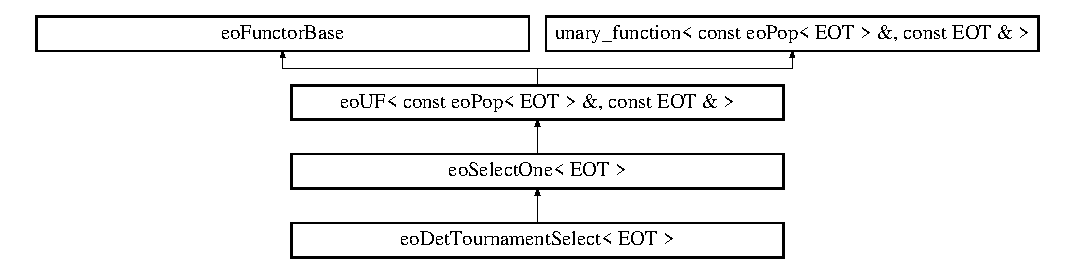
\includegraphics[height=3.23699cm]{classeo_det_tournament_select}
\end{center}
\end{figure}
\subsection*{Public Member Functions}
\begin{CompactItemize}
\item 
{\bf eo\-Det\-Tournament\-Select} (unsigned \_\-t\-Size=2)\label{classeo_det_tournament_select_a0}

\item 
virtual const {\bf EOT} \& {\bf operator()} (const {\bf eo\-Pop}$<$ {\bf EOT} $>$ \&\_\-pop)\label{classeo_det_tournament_select_a1}

\begin{CompactList}\small\item\em The pure virtual function that needs to be implemented by the subclass. \item\end{CompactList}\end{CompactItemize}
\subsection*{Private Attributes}
\begin{CompactItemize}
\item 
unsigned {\bf t\-Size}\label{classeo_det_tournament_select_r0}

\end{CompactItemize}


\subsection{Detailed Description}
\subsubsection*{template$<$class EOT$>$ class eo\-Det\-Tournament\-Select$<$ EOT $>$}

eo\-Det\-Tournament\-Select: a selection method that selects ONE individual by deterministic tournament -MS- 24/10/99 



Definition at line 44 of file eo\-Det\-Tournament\-Select.h.

The documentation for this class was generated from the following file:\begin{CompactItemize}
\item 
eo\-Det\-Tournament\-Select.h\end{CompactItemize}
